\begin{frame}{Présentations}
  Présentez-vous à un.e voisin.e.
  Dites-lui votre \alert{nom}, d'\alert{où} vous venez et votre \alert{majeure}.
  Rappelez-vous ces renseignements pour les présenter à la classe après.
  \alert{Important}: écrivez le \emph{prénom} de votre voisin.e sur un petit papier.
  \begin{columns}
    \column{0.2\textwidth}
      \begin{center}
        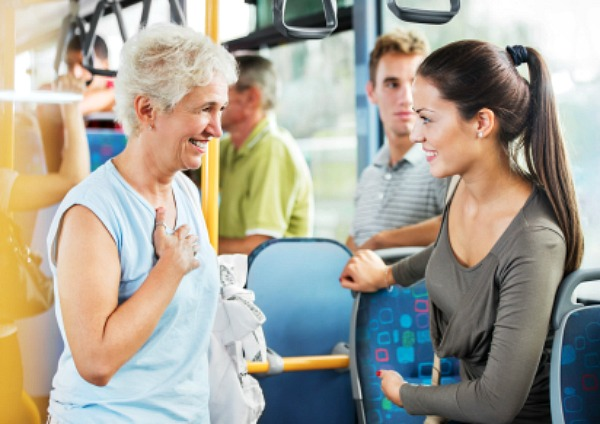
\includegraphics[scale=0.15]{politesse.jpg}
      \end{center}
    \column{0.8\textwidth}
      \uncover<2->{
      \begin{center}
        \begin{tabular}{l @{ $\to$ } l}
          \gloss{What is your name?}  & \uncover<3->{Comment t'appelles-tu?} \\
          \gloss{Where are you from?} & \uncover<4->{D'où viens-tu?} \\
          \gloss{What is your major?} & \uncover<5->{Quelle est ta majeure?} \\
        \end{tabular}
      \end{center}
      }
  \end{columns}
\end{frame}